\section{Methods} \label{SciRob:sec:methods}

\begin{figure}
    \centering
    \includegraphics[width=0.8\linewidth]{Chap2/images/figure2}
    \caption{Pictures of our simulation and real robot scenarios. (A) Simulated Rope Dragging. (B) Simulated Tabletop Rope Manipulation. (C) Retrieving a Charging Cable. (D) Removing Lifting Straps. (E) Moving a Hose. (F) Preparing to Install a Hose. Annotations show examples of goals for various tasks our method can complete.}
    \label{Scirob:fig:figure2}
\end{figure}


\subsection{Data Collection for Learning the Dynamics}

\label{Scirob:sec:phase_one_collection}
Our first phase of data collection is used for training our model of the unconstrained dynamics. This involves sampling random actions and recording the observed states to form trajectories $[\state^0,\action^0,\state^1,\dots,\lasttrainaction,\lasttrainstate]$. In all our experiments, we use $\trainhorizon=10$. We sample actions randomly, choosing target positions which are within \SI{0.1}{\meter} of the current gripper position(s). Put another way, we sample actions which are changes in position in a ball around the current position. We repeat the previously sampled change in position with 80\% probability, which creates larger, more consistent motions and gives better coverage of our environments. During this phase, we do not reset the rope's position between trajectories.

In this phase, we also want to avoid activating physical constraints during data collection. This is done by removing obstacles, and by restricting the actions taken during data collection. For rope dragging, this only means removing any obstacles. For dual arm rope manipulation, this means removing obstacles, removing the arms entirely, and preventing the rope from overstretching by limiting the distance between the grippers. Although removing the arms would not be possible in the real world, it seems possible to design a conservative set of actions which would similarly ensure that the rope does not interact with the arms, or the arms with each other. At a high level, the purpose of this is to simplify the dynamics by avoiding activating any physical constraints during this phase.

For rope dragging, we collected 6,144 trajectories containing 10 steps, of which 1,536 are reserved for validation and testing. For dual arm rope manipulation, we collected 2,048 trajectories containing 10 steps, of which 512 are reserved for validation and testing.
\subsection{Learning the Unconstrained Dynamics}
\label{Scirob:sec:learning_dynamics}

Once we have collected our dataset of trajectories, we train our dynamics network. This network is a two layer fully connected neural network which takes in a state $\currentstate$ and action $\currentaction$ and predicts a change in state $\Delta \nextstatepred$. A diagram showing this architecture is shown in Figure \ref{Scirob:fig:figure4} and discussed in more detail in Section ``\nameref{Scirob:sec:architectures}''. This model can be used to make multistep predictions by feeding the predicted state back into the model. The loss is the combined prediction error for all time steps in the trajectory, and is shown in Equation \eqref{Scirob:eq:dyn_loss}.

\begin{equation}
	\begin{split}
	MSE(\state^0, \action^0, \dots, \lasttrainaction) &= \frac{1}{\trainhorizon} \sum_{t=1}^{\trainhorizon-1} \left\| \currentstatepred - \currentstate \right\|^2 \\
	\statepred^0 &= \state^0 \\
	\nextstatepred &= \ourdynamics(\env, \currentstatepred, \currentaction)
	\end{split}
	\label{Scirob:eq:dyn_loss}
\end{equation}

\subsubsection{Incorporating Uncertainty in the Learned Dynamics}
\label{Scirob:sec:uncertainty}

Prior work has shown that it can be beneficial to consider the uncertainty in the learned dynamics \cite{Schneider1996,Bechtle2019,Chua2018}, even without considering constraints not seen in training. For instance, if the training data does not cover the state-action space well, then having a measure of uncertainty in the dynamics predictions makes it possible to detect out of distribution predictions. This is a measure of \textit{epistemic uncertainty}---uncertainty due to lack of data (as opposed to inherent randomness) \cite{Hullermeier2021,Hora1996}.

As is done in prior work \cite{Gal2016,Chua2018,Lakshminarayanan2017}, we use an ensemble of neural networks trained on the same phase one data starting with different random seeds. When a point prediction is needed, like in planning or in constructing the classifier and recovery datasets, we take the mean of the ensemble prediction. When a measure of uncertainty is needed, we compute the sum of the standard deviations along each dimension of state across all the models in the ensemble. For simplicity we will denote this as $\variance$. We use this measure of uncertainty as an input to the classifier. The intuition behind this method is that the trained networks' predictions will be similar near the training data, but will diverge far away from training data. This makes it possible for the classifier to reject or accept transitions based on the uncertainty of the learned dynamics. Although we did not find that this provided a significant improvement for our tasks, we include it nonetheless as it may be beneficial in scenarios where the unconstrained model is trained on a dataset with poor coverage of the state space.

\subsection{Phase Two Data Collection}
\label{Scirob:sec:phase_two_collection}

Once the unconstrained dynamics have been learned, we next learn where this model is accurate, and what actions to take when it is not. For this, we perform a second phase of data collection. In this phase, we collect data in the kinds of environments where we intend to perform tasks. We perform the same type of random data collection process as in the first phase, but now physical constraints are included, allowing us to gather examples of where our unconstrained dynamics are accurate and where they are not. Using the data collected in this phase, we can construct datasets to train our classifier as well as our recovery actions model. A related approach was used in \cite{Guzzi2020} for learning to estimate the reachability of a quadruped robot. Our prior work has also demonstrated that this type of data can also be collected by planning and executing those plans, rather than by taking random actions \cite{McConachie2020}. However, both of the above methods used analytical/simulation models for predicting the dynamics. Furthermore, our approach is in contrast to many methods in robust control and safe reinforcement learning, which are built on the idea that predictions made outside the training distribution are unreliable \cite{Zhou1998,Gal2016}. Those methods do not require a second data collection phase, but as a consequence would be overly conservative as the presence of any obstacle near the rope would be considered out-of-distribution.

In order to get diverse data we frequently randomize the locations of obstacles in the environment. For dual arm rope manipulation, this requires releasing the rope and moving the arms out of the way before randomizing obstacles, so that we can arrange the obstacles without permanently entangling the rope or arms.

For rope dragging, we collected 2,048 trajectories of length 50 in phase two, of which 512 were reserved for validation and testing. For dual arm rope manipulation, we collected 5,996 trajectories of length 20, of which 1,516 were reserved for validation and testing.

In total, the combined phase one and two datasets for dragging has 163,840 transitions, and the combined phase one two datasets for dual arm rope manipulation has 140,400 transitions. In comparison, \cite{Propnet} uses 500,000 transitions in order to accurately learn the contact dynamics of a rope amongst disc-shaped obstacles in 2D.

\subsection{Learning the Classifier}
\label{Scirob:sec:learning_classifier}

Given the data collected in phase two, we now describe how to construct training examples for the classifier. For this we need both the predictions of the unconstrained dynamics as well the labels of whether the model-error requirement is satisfied. To compute the predictions, we take the starting state for each trajectory in the dataset and roll out the unconstrained dynamics prediction for the rest of the trajectory. This produces a tuple of $(\currentstate, \currentstatepred, \currentaction, \nextstate, \nextstatepred)$ for each time step in each trajectory. As stated in Problem $\eqref{Scirob:eq:planning_problem}$ the label should be 1 if $\modelerrorconstraint$ and 0 otherwise. To compute $\modelerror$, we require a distance function $\distfname$ between the predicted state $\nextstatepred$ and the actual state $\nextstate$. We selected the threshold $\modelerrorthreshold$ by computing the 90th percentile of prediction error for the unconstrained dynamics on the unconstrained dynamics validation set. A sensitivity analysis of the threshold is given in Supplementary Materials. For rope dragging, $\modelerrorthreshold=$\SI{0.065}{\meter} and for dual arm rope manipulation $\modelerrorthreshold=$\SI{0.025}{\meter}. Additionally, we discard all the transitions after the first transition labeled 0, since it is unclear whether the dynamics would have been accurate had it not diverged previously. A diagram illustrating how a trajectory is converted into examples for the classifier is shown in Figure \ref{Scirob:fig:3DClassifierInput}.

\begin{figure}
    \centering
    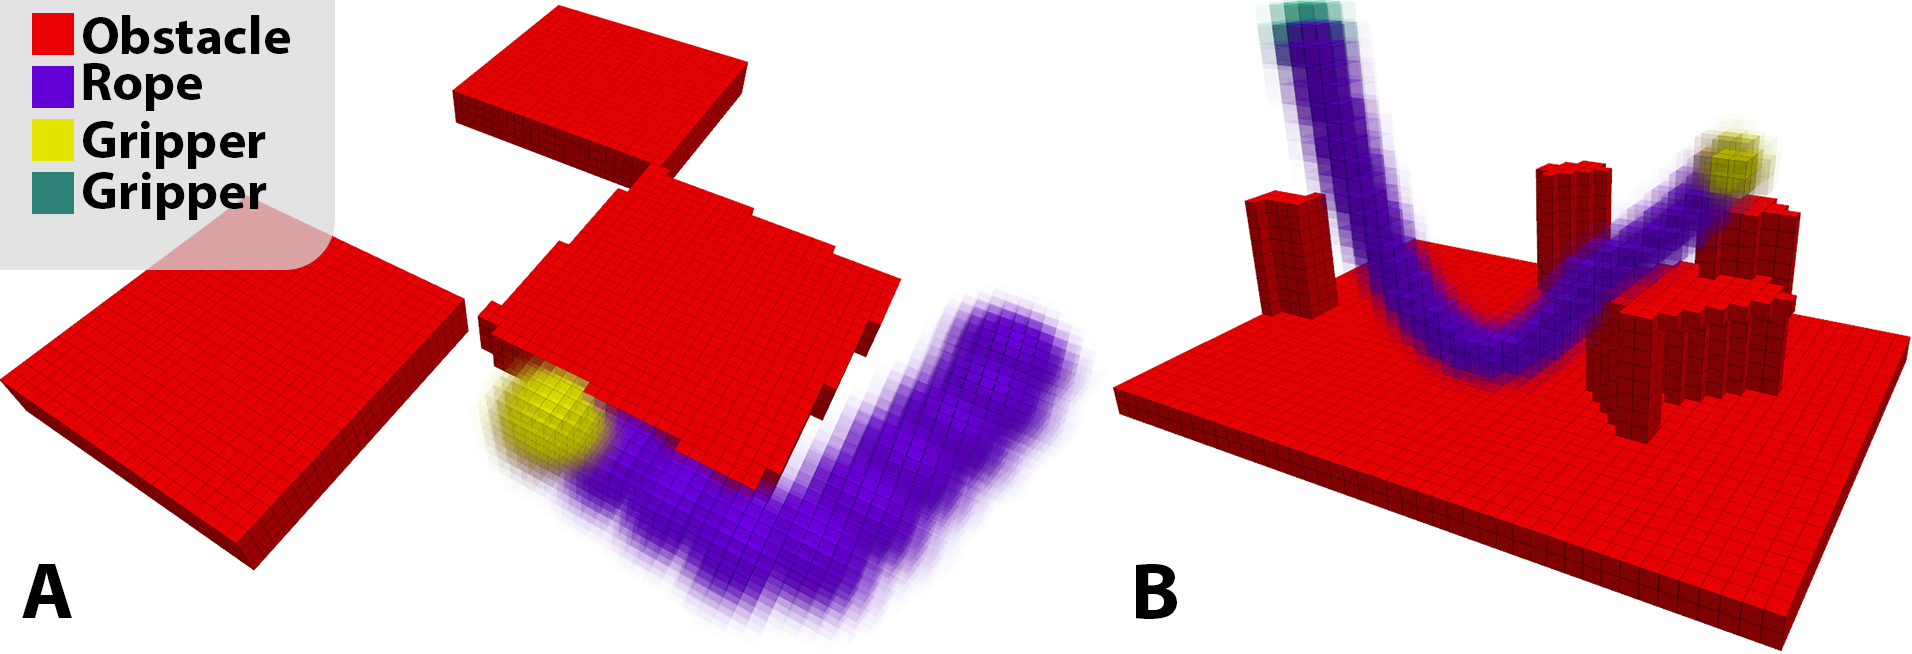
\includegraphics[width=0.6\linewidth]{Chap2/images/figure5}
    \caption{Representing the state and environment in 3D voxel grids. (A) An example for rope dragging. (B) An example dual arm rope manipulation. Different colors are used to represent different channels in the voxel grid, and alpha is used to indicate the voxel value, with 0 being fully transparent and 1 being fully opaque.}
    \label{Scirob:fig:3DClassifierInput}
\end{figure}

The classifier network $\classifierdef$ takes as input the environment $\env$ and the transition $\currentstatepred,\currentaction,\nextstatepred$. Since we use an ensemble of dynamics models, these states are the mean predictions of the ensemble. We also include the variance $\variance$ of the ensemble predictions as input to the classifier. The classifier outputs a number between 0 (inaccurate) and 1 (accurate). The network architecture is shown in Figure \ref{Scirob:fig:figure4}. Since this is a binary classification problem, we use binary cross-entropy loss to train it. Furthermore, since physical constraints are spatial in nature, we convert the environment and states into multi-channel 3D voxel grids and use Convolutional Neural Networks (CNN) (details in Section ``\nameref{Scirob:sec:architectures}'').

We also note that depending on the environments and specific parameters for how actions are sampled, the resulting dataset of transitions may be imbalanced. In our experiments, our classifier datasets contained more positive than negative examples, ranging between 65\% and 95\% positive. To mitigate bias in our classifier, we balance each minibatch by oversampling examples from the underrepresented class.

\subsection{Planning With a Learned Model and Classifier}
\label{Scirob:sec:planning}

Once we have learned our unconstrained dynamics and classifier, these models are used for planning. Although they could be applied to a number of different planning methods, including the cross entropy method (CEM) \cite{Kobilarov2011}, probabilistic roadmaps (PRM) \cite{Kavraki1996}, or trajectory optimization \cite{Ratliff2006}, we chose to use them in a kinodynamic RRT \cite{LaValle2001}, as implemented in the Open Motion Planning Library (OMPL) \cite{ompl}. Kinodynamic RRT is a sampling-based tree-search algorithm, and is well suited for our tasks as they contain local minima and narrow passages. Graph-based methods like PRMs could be used instead if we expect to plan repeatedly in the same environment, and trajectory optimization could be used if there are criteria such as path length which should be minimized.

In our Kinodynamic RRT, we sample a single random action $\currentaction$ and attempt to extend using that action. Whenever we attempt to extend from state $\currentstatepred$ with action $\currentaction$ to the state $\nextstatepred$, we first check the transition $(\currentstatepred,\currentaction,\nextstatepred)$ by feeding it through the classifier. The extension is added to the tree only if the classifier output is greater than $\paccept$. We chose this type of planner for its simplicity, and many algorithmic and implementation optimizations could be made to decrease planning times.

\subsection{Evaluating Stuck States and Learning Recovery}
\label{Scirob:sec:learning_recovery}

The formal definition of being stuck (Equation \eqref{Scirob:eq:recovery}) evaluates every possible action from a given state. In practice, checking whether a state is stuck consists of sampling $\NRecoverySamples$ actions and checking whether any of them are accepted by the classifier. Since the classifier is trained to approximate the MER, this is a quick and effective method for determining whether recovery is needed. Additionally, this procedure is done naturally by the RRT at the start of planning, which means that checking for recovery can be easily integrated into planning without any redundant calls to sampling, dynamics, or classification.

Given the unconstrained dynamics and the classifier, we can also use the data collected in phase two to learn recovery actions. As defined in our problem statement, recovery actions are needed when the robot is in a state where the classifier rejects all proposed actions. In this case, we would like the robot to take \textit{recovery actions} which bring it back to regions of state space where the unconstrained dynamics are accurate.

For this, we propose training a neural network to evaluate the probability that an action is recovering. This network takes in a state, action, and the environment $\recovInputs$ and outputs the probability $\recovProb$ that the action is recovering. Specifically, when we detect recovery is needed, we sample $\NRecoverySamples$ actions randomly and use this learned recovery model to assign each action a probability of recovering. The highest probability action is then selected and executed; this sampling, recovery probability evaluation, and execution process repeats until the system is no longer stuck. This approach requires training a model which estimates the probability that an action is recovering. To construct a dataset of recovering actions and labels of the recovery probability, we use a similar approach to the one used to construct the classifier dataset.

This process considers each observed transition $\currentstate,\currentaction,\nextstate$ and environment $\env$ in the dataset and first determines whether recovery is needed at $\currentstate$. We sample $\NRecoverySamples$ random actions from that state, predict according to the unconstrained dynamics, and feed this into the classifier. If all $\NRecoverySamples$ sampled transitions are rejected, then the state $\currentstate$ needs recovery. Next we perform the same test starting at the next state $\nextstate$. Here we record the proportion of the sampled actions which were accepted, and this is used as the label for probability of recovery $\recovProb$. For example, if at $\currentstate$ none of the random samples were accepted, but from $\nextstate$ all $\NRecoverySamples$ were accepted, then this is an excellent example of recovery, and we would like our recovery model to predict that taking action $\currentaction$ from $\currentstate$ in environment $\env$ is likely to lead to recovery. On the other hand, if when checking $\nextstate$ we find that still no actions are accepted by the classifier, then this is a poor example of recovery. We use all transitions for which recovery is needed (i.e. $\recoveryfuncfull = 1$ as the dataset for training our recovery model, and train the network using binary-cross entropy to predict the recovery probability. For our experiments, we set $\NRecoverySamples$ to 32. More details about the neural network and its structure can be found in Section ``\nameref{Scirob:sec:architectures}''.

Approaches to recovery like those from the safe exploration community \cite{Koller2018,Berkenkamp2017,Fisac2019safety} are focused on staying within a region of the state space from which the agent can guarantee safety during the learning process, or the existence of a sequence of control actions which will move the system into a predefined safe set. In contrast, our method is targeting the case where the model is already too unreliable for use at the given state and any predictions made cannot be trusted.

\subsection{Network architectures}
\label{Scirob:sec:architectures}

\begin{figure}
    \centering
    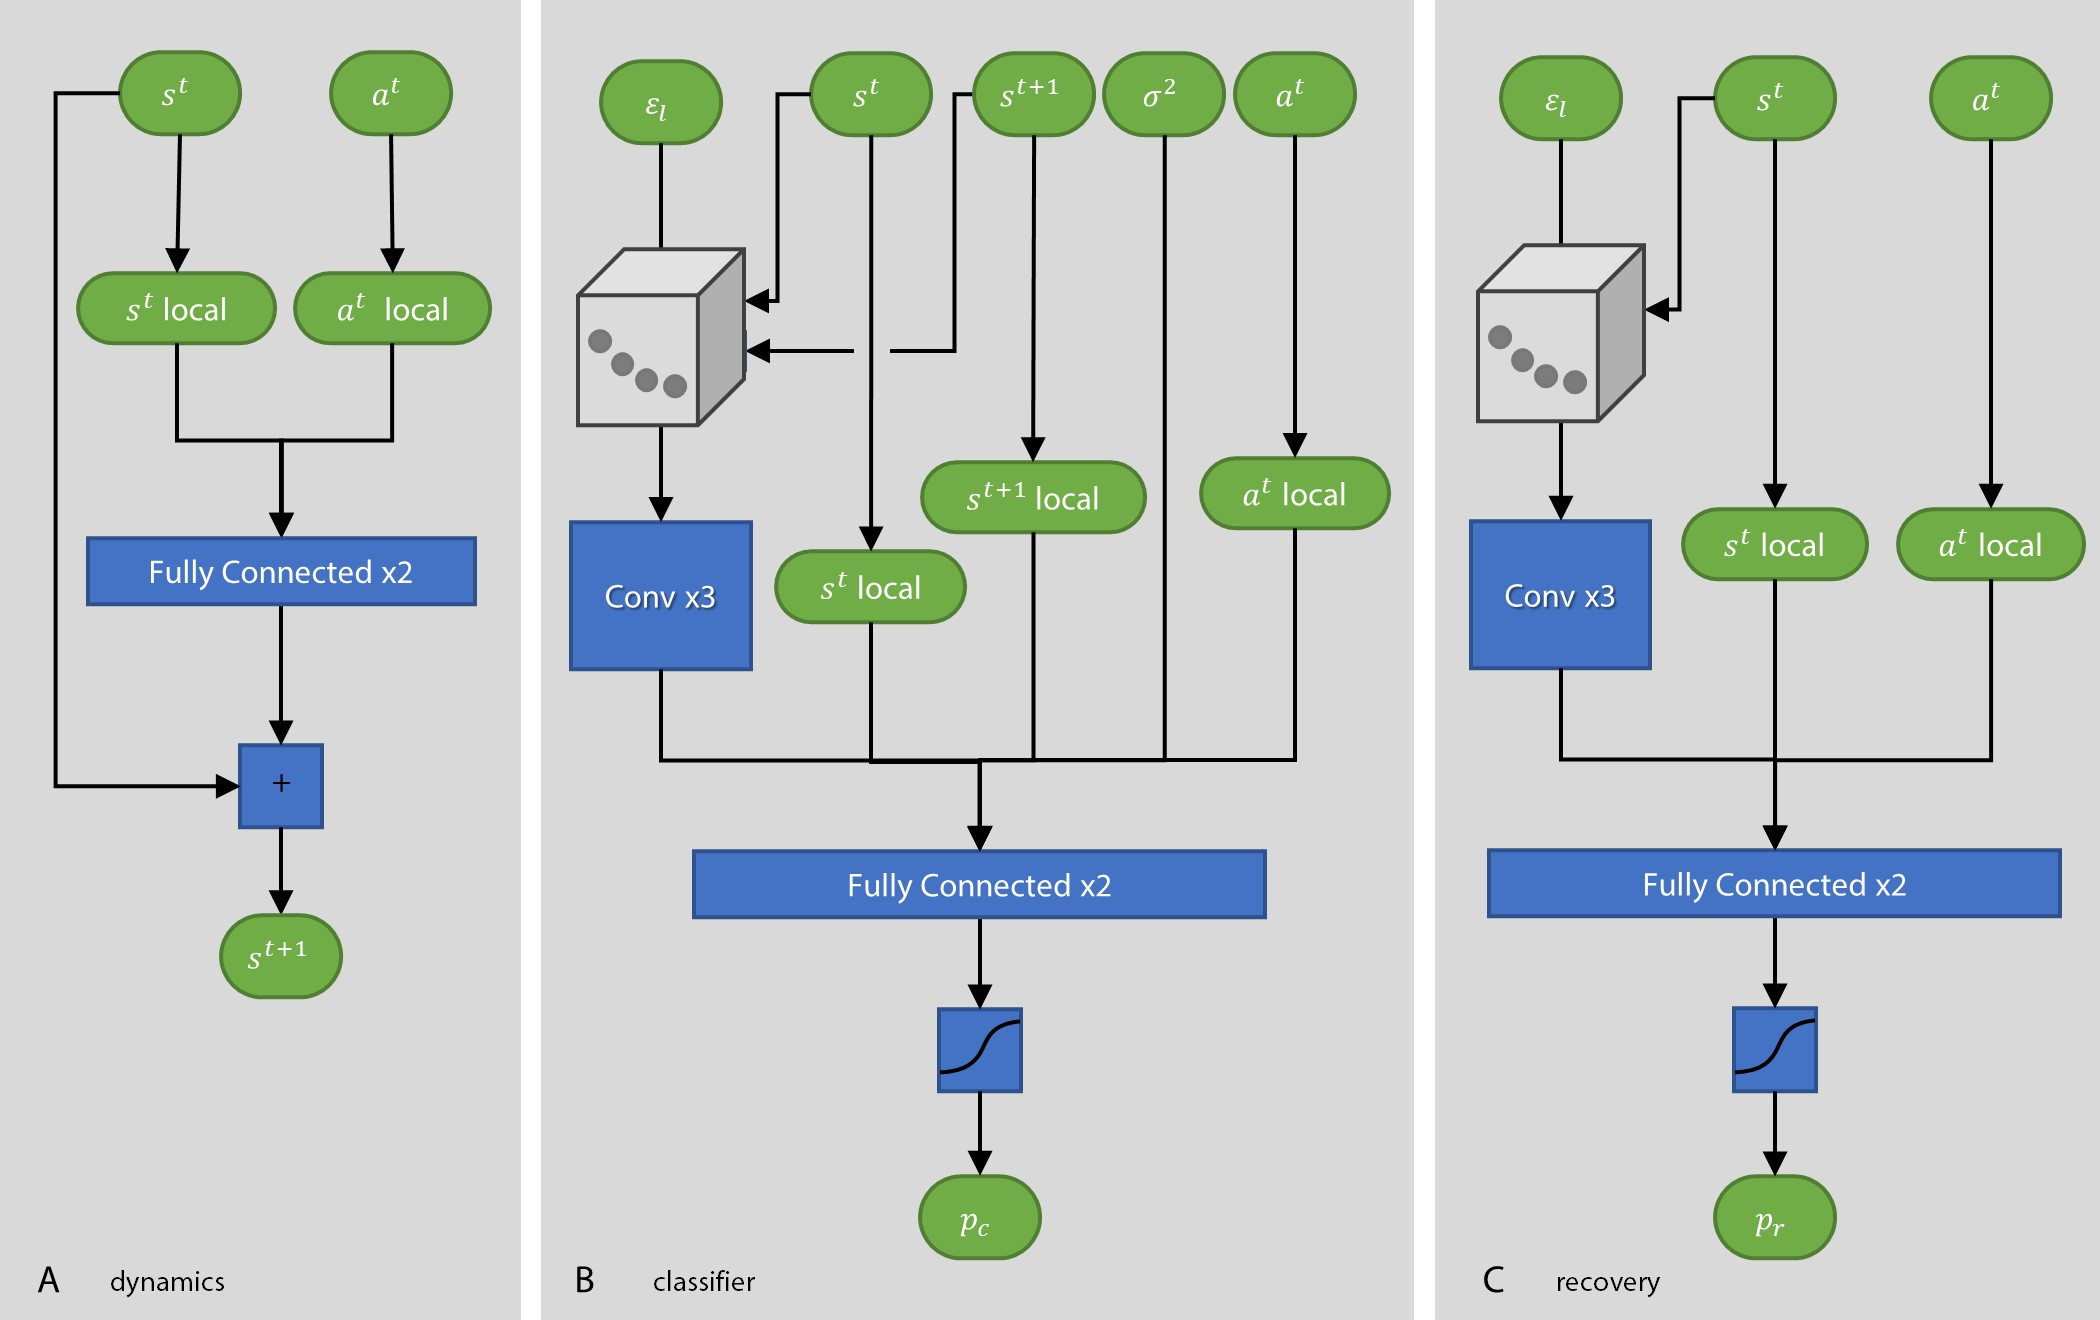
\includegraphics[width=0.7\linewidth]{Chap2/images/figure4}
    \caption{Network architectures. (A) dynamics, (B) classifier, and (C) recovery. \textit{local} refers to the translations used to make the states and actions invariant to the position in the world frame, and is described in Sections ``\nameref{Scirob:sec:learning_dynamics}'', ``\nameref{Scirob:sec:learning_classifier}'', and ``\nameref{Scirob:sec:architectures}''. Green capsules shapes indicate vectors, and blue boxes indicate functions. The gray 3D box represents the 3D voxel grid representation of state (Section ``\nameref{Scirob:sec:voxels}'').}
    \label{Scirob:fig:figure4}
\end{figure}

Our method uses three neural networks, one for the dynamics model, one for the classifier, and one for recovery. Architectures are shown in Figure \ref{Scirob:fig:figure4}.

\subsubsection{Dynamics Model Architecture}

The dynamics network is a two layer fully connected network with 1,024 hidden units in each layer and ReLU activation. This model takes in the state of the rope and grippers concatenated with the actions and outputs the change in state, which is then added to the input state to produce the final predicted state. Furthermore, because we assume that the unconstrained dynamics are invariant to the global position in space, we first translate the state and actions into a local frame before feeding them into the dynamics network. For rope dragging, states and actions are relative to the position of the gripper, and for dual arm manipulation they are relative to the average of all the points of the rope. 

\subsubsection{Classifier Architecture}

The classifier network takes in the environment $\env$ and a transition $\transitionpred$ and outputs the probability of the MER being satisfied. Since we experimented with performing classification on multiple transitions we use a Long Short Term Memory network (LSTM) with a CNN encoder, although in this work we only consider a single transition as input. As shown in Figure \ref{Scirob:fig:figure4}, a single time step is passed through a CNN encoder that maps a single state $\currentstatepred$ and action $\currentaction$ into a latent vector. The state and environment are first represented in a 3D voxel grid and passed through three convolutional layers. The output is flattened and concatenated with the vector representations of the state and action. The LSTM outputs a scalar prediction of the probability of the MER being satisfied for each time step. Since we use a single transition, this means there are two outputs, one for time $t$ and one for $t+1$. The output for time $t$ is ignored, because it is not a function of $\nextstatepred$. Instead, we use the output for time $t+1$ as the probability for the entire transition $\transitionpred$.

\label{Scirob:sec:voxels}
In order to represent the environment and states in a voxel grid of a fixed size, we take a crop of the full environment occupancy grid centered around the local origin (as defined above for dynamics). As with the local representation of states and actions, this assumes invariance to the absolute position. Additionally, using a fixed size local environment has the benefit of allowing the size of the full environment to change from task to task without any retraining. In order to make it easier for the classifier to reason over the 3D input, we also include a 3D representation of the input states. For each component of the state (grippers, rope) we construct a 3D voxel grid of the same size and location as the local environment and each voxel's value is proportional to the inverse-log of its distance to the nearest point in that component of the state. This results in a smoothed version of simply drawing the points into the voxel grid, and examples are shown in Figure \ref{Scirob:fig:3DClassifierInput}. We stack these representations along with the local environment to get a multi-channel voxel grid.

The vector representations of state and action are the same as is described for the dynamics, however we use both the original state vector (not translated) and the local state vector (translated). This is because the classifier should be able to learn reachability and kinematic constraints, e.g. in our dual-arm manipulation scenario. 

\subsubsection{Recovery Architecture}

Finally, the recovery network has the same encoder structure as the classifier, and we use the learned parameters, without fine-tuning, of convolution layers from the classifier in the recovery network. This network takes in a proposed transition, this time consisting of the 3D local environment, a single state, and a proposed action, and outputs the probability of recovery. Unlike the classifier, we do not pass in the predicted result of the proposed action, since recovery is only used when accurate predictions cannot be made. After encoding, two fully connected layer with ReLU activation followed by a layer with sigmoid activation are used to map down to the output probability.

\subsubsection{Full Dynamics Architecture}

Our full dynamics baseline uses a different network. We use the network proposed in \cite{NagabandiImageConditiondDynamics2018}, but extend to 3D convolution. The state representations used are the same as in our unconstrained dynamics network. Graph neural network architectures for predicting physics in 3D may provide more accurate predictions \cite{Propnet,Mrowca2018}, however these networks assume a graphical model of the world is known, whereas our dynamics learning method does not.

\subsection{Simulation Environments}
\label{Scirob:sec:sim_envs}

We use the Gazebo simulator with ODE physics \cite{Gazebo,ODE} for our quantitative experiments. We emphasize that our method does not have access to the simulator's model of the rope or the simulation parameters. For our rope dragging experiment, the rope is modeled with 10 rigid links, and the state consists of the positions of the links and the position of the gripper $\state=[x_g,y_g,z_g,x_1,y_1,z_1,\dots,x_{10},y_{10},z_{10}]$, which has 33 dimensions.
We considered including gripper orientation, however this would make the dynamics dependent on gripper geometry and friction properties (because the rope could wind around the gripper) without necessarily enabling significant new capabilities, so we chose not to include orientation. The gripper is attached to one end of the rope, and the point at the other end of the rope (which we will call the tail) is the point which we wish to place at a goal position. Task error is measured is the Euclidean distance in 3D between the tail and the goal point. The actions are target gripper positions $\action = [x,y,z]$, and a local controller is used to attempt to reach these goals. When commanded into an obstacle, the gripper will stop or potentially slide as it applies force into the obstacle. An action completes when the commanded position is reached or a timeout of 1 second occurs. The nominal joint velocity of the controller is tuned to reduce jerk and keep the simulation quasi-static.

For the dual arm rope manipulation experiments, the rope is modeled with 25 rigid links, and the state consists of the positions of the links and the positions of the two grippers $\state=[x_{g1},y_{g1},z_{g1},x_{g2},y_{g2},z_{g2},x_1,y_1,z_1,\dots,x_{25},y_{25},z_{25}]$, which has 81 dimensions.
The grippers attach to opposite ends of the rope. The actions are target positions for each gripper $\action = [x_1,y_1,z_1,x_2,y_2,z_2]$. A Jacobian-based inverse kinematics controller is used to track the target position for each gripper. This controller stops when the target position is reached or just before any collisions between the arms or between the arms and obstacles.